\documentclass{winnower}
\usepackage{indentfirst}
\usepackage{graphicx}
\usepackage{caption}
\usepackage{subfigure}
\usepackage{xcolor}
\usepackage{float}
\usepackage[section]{placeins}
\usepackage{multirow}
\usepackage{booktabs}
\setlength{\belowcaptionskip}{-0.5cm}

\begin{document}

\title{Homework3 report}

\author{Haoyu Guan}

\affil[1]{Questrom School of Business, Boston University}







\date{2020.02.11}

\maketitle




%-------------------------------------------------%
\section{Problem Backgroud}
%-------------------------------------------------%


\indent \textbf{Option Pricing via FFT Techniques The Heston Model is defined by the following system of stochastic differential equations:}
$$dS_t=rS_tdt+\sqrt{\nu_t}S_tdW_t^1$$
$$d\nu_t=\kappa(\theta-\nu_t)dt+\sigma\sqrt{\nu_t}dW_t^2$$
$$Cov(dW_t^1,dW_t^2)=\rho dt$$

\textbf{The characteristic function for the Heston Model is known to be:}

$$\omega(u)=\dfrac{exp(iu\ln{S_0}+iu(r-q)t+\dfrac{\kappa\theta t(\kappa-i\rho\sigma u)}{\sigma^2})}{(\cosh{\dfrac{\lambda t}{2}}+\dfrac{\kappa-i\rho\sigma u}{\lambda}\sinh{\dfrac{\lambda t}{2}})^{\frac{2\kappa\theta}{\sigma^2}}}$$
$$\Phi(u)=\omega(u)\exp{(\dfrac{-(u^2+iu)\nu_0}{\lambda\coth{\frac{\lambda t}{2}}+\kappa-i\rho\sigma u})}$$
$$\lambda=\sqrt{\sigma^2(u^2+iu)+(\kappa-i\rho\sigma u)^2}$$

\textbf{Assume the risk-free rate is 2$\%$, the initial asset price is 250 and that the asset pays no dividends}

\section{Problem Detail}
\textbf{(a) Exploring FFT Technique Parameters Consider a European Call Option with strike 250 expiring in six months. Additionally, assume you know that the parameters of the Heston Model are:}
$$\sigma=0.2$$
$$\mu_0=0.08$$
$$\kappa=0.7$$
$$\rho=-0.4$$
$$\theta=0.1$$

\textbf{i. Calculate the price of the European Call option with many values for the damping factor, ��. What values of �� seem to lead to the most stable price?}

\begin{figure*}[!h]
\begin{center}
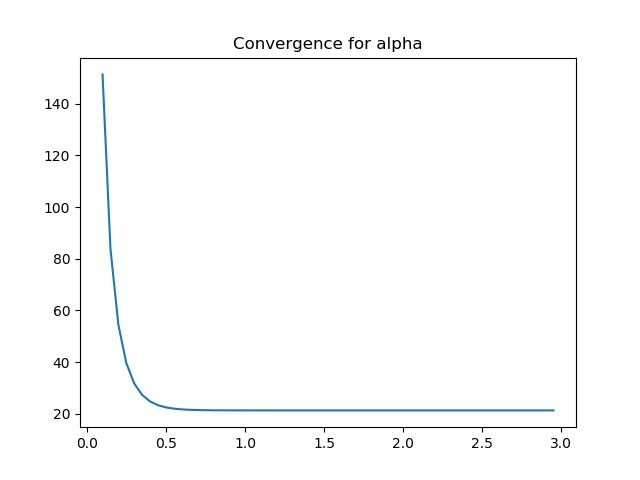
\includegraphics[scale=0.6]{1_1.jpg}
\caption
{Convergence for alpha}
\label{fig:f1}
\end{center}
\end{figure*}



The price of the call option is 21.274373625509146. We can see the picture.When $b=S_0+S_0*7*\sigma$.If $\alpha>1.15$,It will be the most stable.So I will choose $\alpha=1.5$ as my choice
\\


\textbf{ii. Using the results above, choose a reasonable value of �� and calculate the price of the same European Call with various values of N and $\Delta k$ (or equivalently N and B). Comment on what values seem to lead to the most accurate prices, and the efficiency of each parameterization.}


\begin{figure*}[!h]
\begin{center}
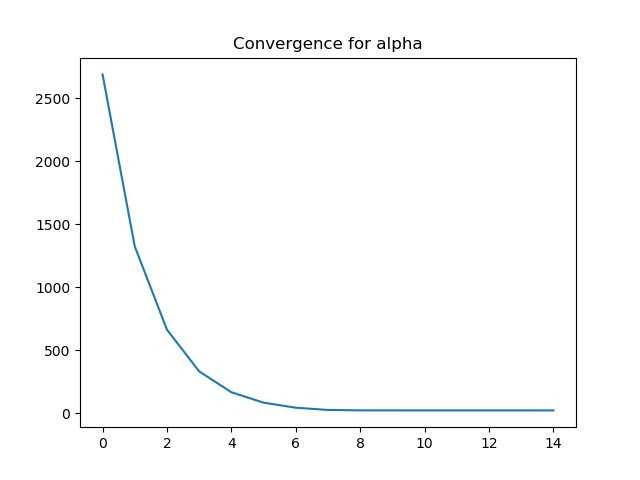
\includegraphics[scale=0.6]{1_2.jpg}
\caption
{Convergence for alpha}
\label{fig:f1}
\end{center}
\end{figure*}

When $b=S_0+S_0*7*\sigma$. I choose $\alpha=1.5$. I consider N have to bigger than $2^7$ to be accurate
\\

\textbf{ iii. Calculate the price of a European Call with strike 260 using various values of N and $\Delta k$ (or N and B). Do the same sets of values for N, B and $\Delta k$ produce the best results? Comment on any differences that arise}

\begin{figure*}[!h]
\begin{center}
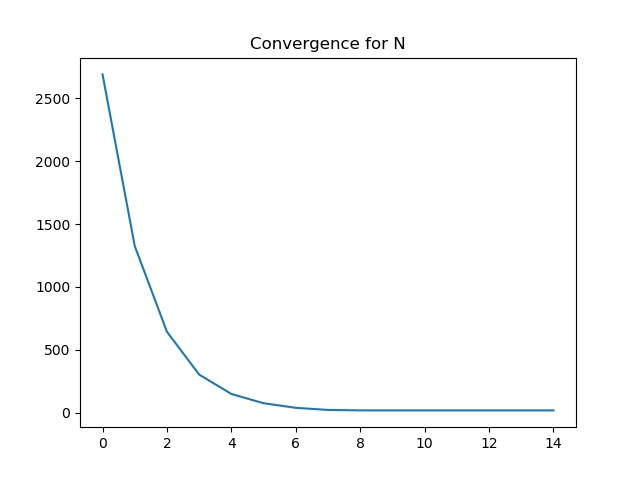
\includegraphics[scale=0.6]{1_3.jpg}
\caption
{Convergence for N}
\label{fig:f1}
\end{center}
\end{figure*}


I think this values of N,B and $\Delta k$ produce the best results
\\

\textbf{(b) Exploring Heston Parameters Assume the risk-free rate is 2.5\%, the initial asset price is 150 and that the asset pays no dividends.}


$$\sigma=0.4$$
$$\mu_0=0.09$$
$$\kappa=0.5$$
$$\rho=0.25$$
$$\theta=0.12$$


\textbf{i. Using these parameters, calculate Heston Model prices for three-month options at a range of strikes and extract the implied volatilities for each strike. Plot the implied volatility $\sigma(K)$ as a function of strike.}
\begin{figure*}[!h]
\begin{center}
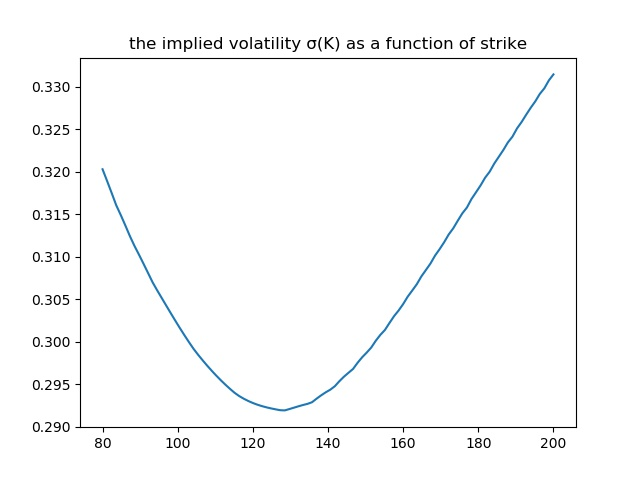
\includegraphics[scale=0.4]{1_4.jpg}
\caption
{$\sigma(K)$}
\label{fig:f1}
\end{center}
\end{figure*}



\textbf{ii. Use the FFT pricing technique to obtain prices of 150 strike calls at many expiries.Extract the implied volatility for each and plot the term structure of volatility by plotting time to expiry on the x-axis and implied volatility on the y-axis.}


\begin{figure*}[!h]
\begin{center}
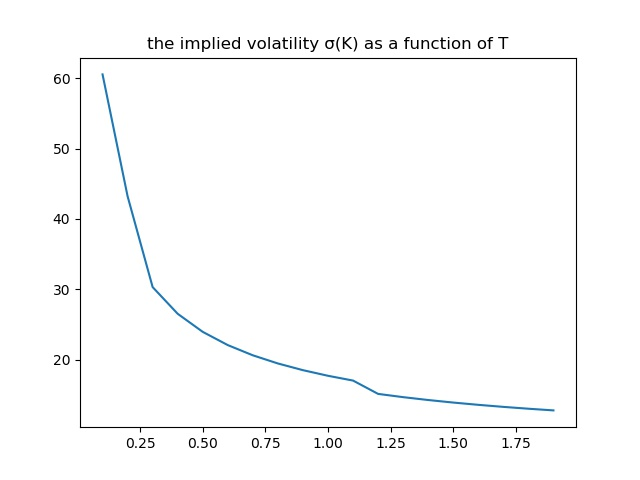
\includegraphics[scale=0.6]{1_5.jpg}
\caption
{$\sigma(T)$}
\label{fig:f1}
\end{center}
\end{figure*}



\textbf{iii. Holding all other para|meters constant, vary each of the model parameters and plot the updated volatility skews and term structures. Comment on the impact that each parameter has on the skew and term structure.}

(1)Change the $\sigma$

\begin{figure*}[!h]
\begin{center}
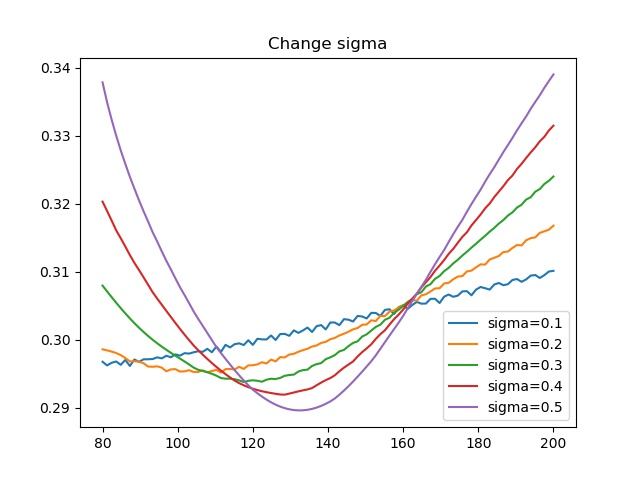
\includegraphics[scale=0.6]{1_6.jpg}
\caption
{Change $\sigma$}
\label{fig:f1}
\end{center}
\end{figure*}


(2)Change the $\nu_0$

\begin{figure*}[!h]
\begin{center}
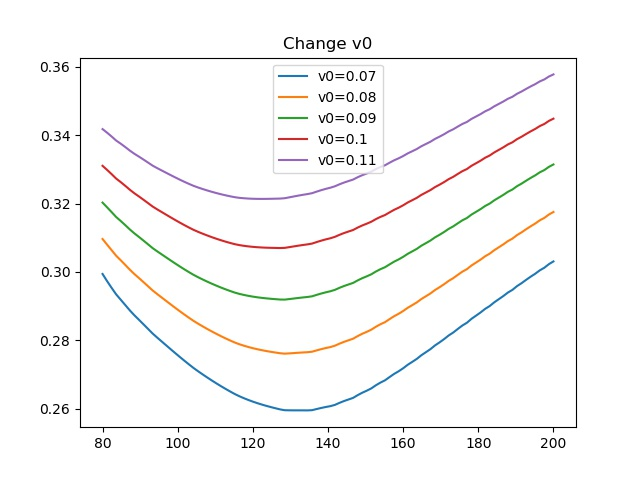
\includegraphics[scale=0.6]{1_7.jpg}
\caption
{Change $\nu_0$}
\label{fig:f1}
\end{center}
\end{figure*}

\newpage
(3)Change the $\kappa$

\begin{figure*}[!h]
\begin{center}
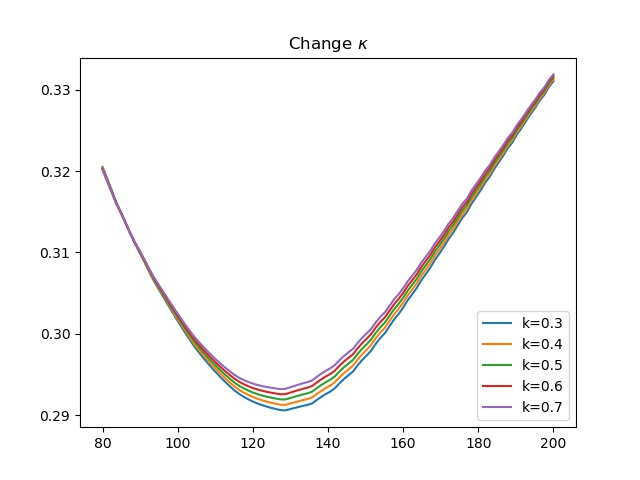
\includegraphics[scale=0.6]{1_8.jpg}
\caption
{Change $\kappa$}
\label{fig:f1}
\end{center}
\end{figure*}

(4)Change the $\rho$

\begin{figure*}[!h]
\begin{center}
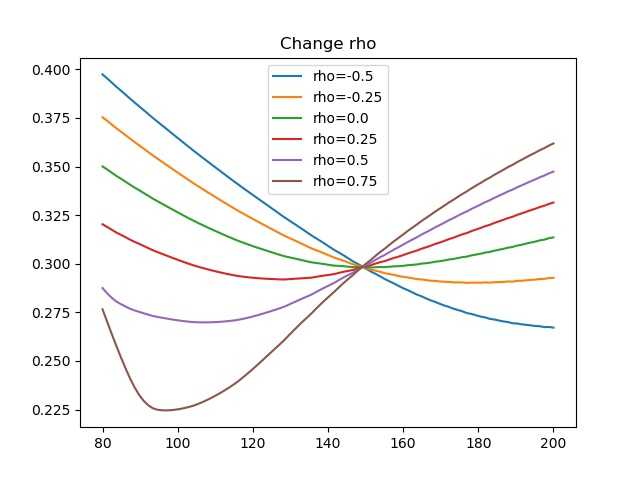
\includegraphics[scale=0.6]{1_9.jpg}
\caption
{Change $\rho$}
\label{fig:f1}
\end{center}
\end{figure*}

\newpage

(5)Change the $\theta$

\begin{figure*}[!h]
\begin{center}
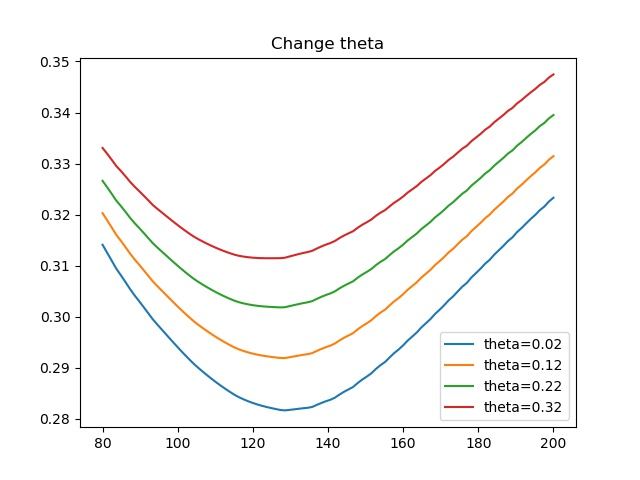
\includegraphics[scale=0.6]{1_10.jpg}
\caption
{Change $\theta$}
\label{fig:f1}
\end{center}
\end{figure*}


\end{document}
